\chapter{Reinforcement learning}
\label{chp:reinforcement_learning}

Having identified reinforcement learning as the solution technique for this project, we give a brief overview of the relevant theory. 
We begin by introducing the precise mathematical problem that reinforcement learning solves, the Markov decision processes (MDP).
We then give a brief overview of the use of neural networks as function approximators as a necessary requirement to practically realise MDPs in large state spaces, followed by a taxonomy of reinforcement learning algorithms. 
We discuss the reinforcement learning algorithms relevant to robotics control, namely those that allow for continuous action spaces in more detail. The discussion on MDPs and RL is adapted from Silver's reinforcement learning course \cite{silver2015} and Sutton and Barto's reinforcement learning textbook \cite{sutton2020}.

\section{Markov decision processes}

The MDP provides a mathematical framework for modelling time discrete decision making processes where the outcomes are partly random and partly under the control of the decision maker, otherwise referred to as the agent. 
The property of the MDP to model partly random sequential problems is useful for the autonomous racing problem, where the outcome of the race is determined by a sequence of control actions, and the exact vehicle dynamics model is not known.
We begin our discussion of MDPs by introducing its formal definition.

\subsection{Formal definition}
\label{sec:mdp_def}

Silver \cite{silver2015} gives the formal definition of the Markov decision process as a tuple $\langle \mathcal{S,A,P,R}, \gamma \rangle$, where 
\begin{itemize}
    \item $\mathcal{S}$ is the set of all environment states,
    \item $\mathcal{A}$ is the set of all actions available to the agent,
    \item $\mathcal{P}$ provides all the possible state transitions:
    \begin{itemize}
        \item $\mathcal{P}_{ss'}^{a} = \mathbb{P} [S_{t+1}=s' |  S_t=s, A_t=a]$,
    \end{itemize}
    \item $\mathcal{R}_{s}^{a} = \mathbb{E} [R_{t+1} | S_t=s, A_t=a]$ is a reward function, and
    \item $\gamma \in [0,1]$ is a discount factor
\end{itemize}
The following sections describe how each of the elements of the tuple are used in the MDP. We begin by discussing the structure of the MDP, i.e., how the agent and environment interact. 

\subsection{The agent environment interface}
\label{sec:agent_environment_interface}
The agent and environment are considered separate entities that interact in a sequence of discrete time steps, $t=0,1,2,3, ...$.
At every time step $t$, the agent observes the environment's state $S_t \in \mathcal{S}$, on which basis it selects an action $A_t \in \mathcal{A}$.
The action is executed, modifying the state according to the state transition probabilities $\mathcal{P}$ in the environment.
The agent receives then receives the next state $S_{t+1}$ and a numerical reward $R_{t+1} \in \mathcal{R} \subset{\mathbb{R}} $ at time step $t+1$. This agent environment action is repeated, giving rise to the trajectory

\begin{equation}
S_0, A_0, R_1, S_1, A_1, R_2, S_2, A_2, R_3, ... .
\label{eq:mdp_trajectory}
\end{equation}

\begin{figure}[!htb]
\centering
\input{contents/chapt3/figs/agent_environment_boundary.pdf_tex}
\caption[The agent environment interface]{The agent environment interface.}
\label{fig:agent_env_boundary}
\end{figure}

\subsection{Rewards and returns}
The goal of the agent is to maximise an expected return $G_t$, defined as the expected sum of rewards from the current time step until the end of the episode,
\begin{equation}
G_t \doteq R_{t+1} + \gamma R_{t+2} + \gamma^2 R_{t+3} + ... = \sum_{k=t+1}^{T} \gamma^{k-t-1} R_{k}.
\label{eq:G_t}
\end{equation}
where $\gamma$ is a discount factor controlling how strongly future rewards are weighted. An important property that reinforcement learning utilises is that the returns at successive time steps can be related to each other:
\begin{equation}
\begin{split}
G_t &= R_{t+1} + \gamma R_{t+2} + \gamma^2 R_{t+3} + ... \\
&= R_{t+1} + \gamma (R_{t+2} + \gamma R_{t+3 + ...}) \\
&= R_{t+1} + \gamma G_{t+1}. 
\label{eq:G_t_recursive}
\end{split}
\end{equation}

\subsection{Policies and value functions}
To solve an MDP, it is necessary for the agent to formulate an action choosing policy $\pi$. That is, a mapping from states to the probability of selecting each action. This is mathematically expressed as
\begin{equation}
\pi(a|s) = \mathbb{P} [A_t=a | S_t=s].
\label{eq:pi(a|s)}
\end{equation}
The goal of the agent is to improve $\pi$ so as to maximise the reward signal. 
This requires a means of evaluating the performance of the policy: the \emph{state-value} function.
Formally, the value of being in a state $s$ while following policy $\pi$ is denoted by state-value $v_\pi$, and is the expected return $G_t$ for the entire episode when starting in state $s$ and following policy $\pi$ thereafter:
\begin{equation}
v_\pi(s) = \mathbb{E}_{\pi} [G_t | S_t=s].
\label{eq:v_pi(s)}
\end{equation}
Closely related to the state-value function is the \emph{action-value function}, denoted $q_\pi$. Formally, the value of taking action $a$ in state $s$ and following policy $\pi$ thereafter is
\begin{equation}
q_\pi(s,a) = \mathbb{E}_{\pi} [G_t | S_t=s, A_t=a].
\label{eq:q_pi(s,a)}
\end{equation}
Equations \ref{eq:v_pi(s)} and \ref{eq:q_pi(s,a)} are sampled in Monte Carlo reinforcement learning techniques.
By substituting Equation \ref{eq:G_t_recursive} into Equation \ref{eq:v_pi(s)} and Equation \ref{eq:q_pi(s,a)}, we are able to relate the state and action values to themselves at the next time step:
\begin{equation}
v_\pi(s) = \mathbb{E}_{\pi} [R_{t+1} + \gamma v_{\pi}(S_{t+1}) | S_t = s],
\label{eq:v_pi(s)_1}
\end{equation}
\begin{equation}
q_\pi(s,a) = \mathbb{E}_{\pi} [R_{t+1} + \gamma q_{\pi}(S_{t+1}, A_{t+1}) | S_t = s, A_t=a].
\label{eq:q_pi(s,a)_1}
\end{equation}
These equations are sampled in temporal difference reinforcement learning techniques discussed later in this chapter and are key to online reinforcement learning. 
For now, we remove the expectation $\mathbb{E}$ from Equations \ref{eq:v_pi(s)_1} and \ref{eq:q_pi(s,a)_1} to obtain the Bellman expectation equations for $v_\pi$ and $q_\pi$, respectively:
\begin{equation}
   v_\pi(s) = \sum_{a \in \mathcal{A}} \pi(a|s) (\mathcal{R}_{s}^{a} + \gamma \sum_{s' \in \mathcal{s}} \mathcal{P}_{ss'}^{a} v_\pi(s')),
   \label{eq:bellExpv}
\end{equation}
\begin{equation}
   q_\pi(s,a) = \mathcal{R}_s^a + \gamma \sum_{s'\in\mathcal{S}}\mathcal{P}_{ss'}^a \sum_{a'\in\mathcal{A}}\pi(a'|s')q_\pi(s',a').
   \label{eq:bellExpq}
\end{equation}
These bellman expection equations more clearly show that both the state-values $v_\pi$ and action-values $q_\pi$ are dependent on the policy $\pi$. Thus, selecting a better policy directly leads to higher values for $v_\pi$ and $q_\pi$. Since quality of a policy is defined in terms of $v_\pi$ and $q_\pi$, we can say that a policy $\pi$ is better than policy $\pi'$ if its expected return is greater than that of $\pi'$ for all states, formally expressed as
\begin{equation}
\begin{split}
    \pi \geq \pi' \text{ if and only if } v_\pi(s) \geq v_{\pi'}(s) \text{ and } \\
    q_\pi(s,a) \geq q_{\pi'}(s,a) \text{ for all } s \in \mathcal{S} \text{ and } a \in \mathcal{A}.
\end{split}
\end{equation}
Now that we have a means of measuring the performance of policies using value functions, we can discuss optimal policies: these are policies which achieve the best performance by maximising the value functions.

\subsection{Optimal policies and value functions}
Solving an MDP means finding an optimal policy $\pi_*$ which achieves more reward than all other policies,
$\pi_* \geq \pi \text{ for all } \pi$. All optimal policies share the same optimal state-value function $v_*$ 
and optimal action-value function $q_*$, defined as 
\begin{equation}
    v_*(s)=\max_\pi v_\pi(s) \text{ for all } s \in \mathcal{S},
\label{eq:v_*(s)}
\end{equation}
\begin{equation}
    q_*(s,a)=\max_\pi q_\pi(s,a) \text{ for all } s \in \mathcal{S} \text{ and } a \in \mathcal{A}.
\label{eq:q_*(s,a)}
\end{equation}
An MDP is considered solved when either the optimal state-value $v_*$ or action-value $q_*$ function is known, which is equivalent to maximising the Bellman Equations \ref{eq:bellExpv} and \ref{eq:bellExpq} over all states.
Reinforcement learning techniques try to solve the MDP and formulate an optimal policy $\pi_*$ by improving the current policy $\pi$ with respect to the either the state or action value function.

\subsection{Summary of Markov decision processes}
This concludes our overview of MDPs.
The autonomous racing problem can be solved using reinforcement learning only once it has been modelled as an MDP. This involves populating the five-tuple described in Section \ref{sec:mdp_def}: $\mathcal{S}$ is the set of valid states on the track, $\mathcal{A}$ are the available control actions, $\mathcal{P}$ are the state transition probabilities according to the vehicle dynamics model, and $\mathcal{R}$ is a reward function that we design so that the agent achieves a fast lap time when it maximises the reward. 

Before moving on to reinforcement learning theory, we must address one assumption that was made in this section.
Up to now, we have only presented cases where there are few enough states that a value can be attached to each state or state-action pair.
The state and action value functions are then lookup tables with every entry corresponding to a state or state-action pair.
In practice, this is often not a reasonable assumption to make, as many tasks require large or continuous state spaces.
Moreover, discretising a continuous state space may result in an infeasible number of states.
Having such a large number of states adds the complexity that each state that the agent encounters will most likely never have been encountered before.
As a necessary requirement to make sensible decisions in such environments, reinforcement learning agents must generalise across similar states, otherwise referred to as \emph{function approximation}.
This is the topic of the next section.


\section{Function approximation}
\label{sec:function_approximation}
The task of the function approximator is to construct an approximation of a function $\hat{f}(x,w) \approx f(x)$
%(e.g., $\hat{q}(s,a) \approx q(s,a)$ or $\hat{v}(s) \approx v(s)$) 
from examples of the output of that function. 
In reinforcement learning, this means learning a state-value function $\hat{v}(s) \approx v(s)$, or action-value function $\hat{q}(s,a) \approx q(s,a)$.
Two common methods are linear combinations of features and artificial neural networks (ANNs), both taken from the field of supervised machine learning.
In particular, ANNs have proven successful for function approximation in the continuous control setting and have significantly contributed to the success of reinforcement learning. 
ANNs are the method of function approximation we consider in our study on the basis that using linear combinations of features results in an infeasible number of parameters to keep in memory, and current state of the art reinforcement learning algorithms for continuous action spaces are developed specifically for ANNs.

\subsection{Artificial neural networks}
\label{sec:ann}
We now present an overview of ANNs, which are powerful non-linear function approximators that take inspiration from biological neural networks.
The discussion is adapted from Goodfellow's Deep Learning textbook \cite{Goodfellow2016} and Ng and Katanforoosh's Deep Learning lecture notes \cite{Ng2019}. 
We start our overview with the artificial neuron, so named because it  loosely models neurons in a biological brain. 

\subsubsection{The neuron}
The neuron is the basic form and building block of ANNs.
It is depicted in Figure \ref{fig:neuron} by the circle marked $z$, and its inputs by the column of circles marked $x_1$ to $x_I$, with a weight parameter $\theta_i$ attached to each input $x_i$. 
The neuron simply applies a non-linear \emph{activation function} to a weighted sum of its input values. 
Although a variety of activation functions are used in practice, Goodfellow et al. \cite{Goodfellow2016} recommends the recitfied linear unit as default. It therefore the function of choice for this study:
\begin{equation}
    f(x) = \text{ReLU}(x) = \max(0, \sum_{i=1}^{I}x_i \theta_i).
    \label{eq:ReLU}
\end{equation}
An ANN is a network of these interconnected neurons. Although several structures are possible for ANNs, we focus our discussion on the feed forward neural network (FNN), a standard ANN architecture for reinforcement learning.
\begin{figure}[htb!]
    \centering
    \input contents/chapt3/figs/neuron.tex
    \caption[A single neuron]{A single neuron $z$ with input connections $x$ weighted by $\theta.$}
    \label{fig:neuron}
\end{figure}

\subsubsection{Feed forward neural networks}
\label{sec:fnn}
The structure of the FNN has neurons organised in layers, with each neuron in a layer forming links with the neurons in the preceding and following layers, as depicted in Figure \ref{fig:neural_network}. 
In an FNN, the input of every neuron in a given layer is connected to the weighted output of every neuron in the preceding layer. Likewise, its output connected to every neuron in the following layer. The input to the first layer is the input to the network, and the output of the final layer is the output of the network.
By combining many simple non-linear units in a networked structure, an FNN is able to approximate complex non-linear functions. In fact, according to the universal approximation theorem, an ANN with an appropriate number of connections can approximate any arbitrary relationship between input and output variables.
Having discussed the structure of the neural network, we review the process by which inputs to the FNN are evaluated, i.e. forward propagation, and the optimisation process by which the weight parameters are changed so that network performance in improved.

\begin{figure}[htb!]
    \centering
    \input contents/chapt3/figs/neural_network.tex
    \caption[A neural feed forward network]{An FNN with an input later of three units, one hidden later of two units and an output layer of two units. Each neuron in a layer is connected to each neuron in the next layer, so that the layers are fully connected.
    The neural network recieves an input vector $\mathbf{x}=[x_1, x_2, ... x_I]$ and outputs a prediction $\hat{y}$.}
    \label{fig:neural_network}
\end{figure}

\subsubsection{Forward propagation}
The process of evaluating an input $x$ to generate an output $\hat{y} = \hat{f}(x,\theta)$ from the neural network is called forward propagation, 
so called because the input data is fed through the network in the forwards direction only. 
Each neuron in a given layer computes it activation function from neurons in the preceding layer using Equation \ref{eq:ReLU}.
The layers are computed sequentially from first to last. 

\subsubsection{Optimisation}
The FNN should be optimised so that $\hat{f}(x,\theta)$ represents $f(\theta)$ more accurately, referred to as learning. 
Learning is accomplished by gradient descent, which involves adjusting each weight parameter $w$ so as to improve the network performance with respect to a cost function $J(\theta)$. 
In the standard gradient descent approach, the update to each weight is found by computing the partial derivative, or gradient, of the cost function with respect to that weight. The weights are then adjusted slightly so that the cost moves in the decreasing direction:
\begin{equation}
    \theta_{t+1} = \theta_{t} - \alpha \nabla_{\theta_t}J(\theta_t),
    \label{eq:gradient_descent}
\end{equation}
where $\alpha$ is the learning rate, i.e, a scalar controlling the magnitude of the weight updates.
All gradient descent methods are variations of Equation \ref{eq:gradient_descent}.
However, the method we consider for this study is adaptive moment estimation (Adam), introduced by Kingma and Ba \cite{kingma2015}. 
Adam computes adaptive learning rates for each parameter in the ANN by keeping track of a decaying average of past gradients, referred to as the momentum. 
Before we can compute the learning step, we will need a cost function to minimise and a method to compute gradient of the cost function with respect to the network parameters.

\subsubsection{Cost functions}
The aim of gradient descent is to minimise a cost function $J(\theta)$. This cost function is defined in terms of a loss function $\mathcal{L}(\hat{y}, y)$ that measures the error between the FFN predicted output $\hat{y}$ and target examples of the true function $y = f(x)$. 
The choice of loss function we consider in this study is the square error, 
\begin{equation}
    \mathcal{L}(\hat{y},y)=(\hat{y}-y)^2.
\end{equation}
The cost function is then the mean of the squared error (MSE) over all the instances trained on:
\begin{equation}
    J(\mathbf{\hat{y}, y}) = \frac{1}{N} \sum_{i=1}^{N} \mathcal{L}(\hat{y}^i, y^i) = \sum_{i=1}^{N} (\hat{y}^i - y^i)^2.
    \label{eq:cost_function}
\end{equation}
When this cost function is minimised, the neural network output $\hat{y}$ is brought closer to the true values $y$.
Thus, the neural network $\hat{f}(s,\theta)$ becomes a better approximation of the true function $f(x)$.

\subsubsection{Backpropagation}
The gradient descent method of adjusting an ANN's weights requires an estimate of the partial derivative of a cost function with respect to each weight.
The most efficient method for doing this is backpropagation, whereby the partial derivatives are taken with respect to each layer of neurons in a reverse order through the network.
Backpropagation is started by computing partial derivative with respect to the units in the output layer.
By the chain rule, the partial derivatives with respect to the second to last layer is calculated using the last layer.
This process of working out the derivatives from the last to first layers using the chain rule continues, the derivatives of the units in each layer being used to calculate the derivatives in the preceding layer.

\subsection{Summary of function approximation}
In this section, we have highlighted the need for function approximation and introduced neural networks as a means to that end.
We have given a brief overview of the structure of neural networks, as well as the feedforward mechanism by which it evaluates inputs. We have also reviewed the gradient descent method by which the network is optimised to maximise performance.
Looking ahead, we will see that neural networks are not only useful for function approximation, but are also used to represent policies in the case of policy-gradient reinforcement learning methods.
As such, ANNs are essential in understanding the reinforcement learning methods presented in the next section.

\section{Reinforcement learning}
Having introduced the necessary MDP theory, we move on to reinforcement learning, a solution technique for MDPs that achieve optimal policies and value functions by in a computationally feasible manner by interacting with the environment.
We start our discussion with a taxonomy of the reinforcement learning field.

\subsection{A taxonomy of reinforcement learning}
The first and foremost distinction we can make is that between model-free and model-based methods.
Techniques that explicitly reference a state transition model to compute an optimal policy are model-based.
In practice, the model is often used for planning by `looking ahead' to construct a series of future states, from which an optimal set of actions can be selected \cite{moerland2020}.
However, accurate models describing the state transitions in the environment are rarely available, limiting the use case of model-based methods. 
In fact, inaccuracies in the model propagate error into the look ahead which can cause the algorithm to become unstable.
As such, state of the art model-free methods which learn only through sampled environment interactions and select an action based on past experience without referencing a model often outperform model-based methods \cite{seita2019}.

Since the focus of this study is to develop techniques that address issues that occur with learning approaches to autonomous racing due to model inaccuracies, we limit the scope of the project on model-free reinforcement learning. 
Model-free reinforcement learning methods can be classified into three categories: 
\begin{enumerate}
    \item Value-based, 
    \item policy-based, and
    \item actor-critic.
\end{enumerate}
In value-based methods, the policy $\pi$ is directly determined from the action-value function $q$. The goal then is to estimate the optimal action-value function $q_*$, from which the optimal policy $\pi_*$ is obtained. 
Broadly speaking, value-based methods fall into two categories: Monte Carlo methods which require samples of complete episodes to update the value function, and temporal difference methods that utilise `bootstrapped' estimated action-values to relax the requirement of needing complete episodes.

On the other hand, policy-based methods learn a parameterised policy that selects actions without referencing a value function.
Rather, the policy is optimised directly to maximise the return. While policy-based methods tend to be less sample efficient than value-based methods \cite{nachum2017}, they have an advantage over value-based methods in that they allow for continuous action spaces. Purely policy-based methods are analogous to Monte Carlo in that they require samples of complete episodes.

Closely related to policy-based methods are actor-critic methods in which value-based and policy-based methods are combined by retaining both a parameterised policy and a value function. 
The value functions in actor-critics are learned using value-based reinforcement learning, and the policy is updated with respect to the value function.
This allows for continuous action spaces and online updates to both the value-function and policy, making them analogous to temporal difference learning from value-based methods.
While actor-critics are our method of choice, they contain elements from both value-based and policy-based methods.
We therefore give a brief overview of purely value-based and policy-based methods before discussing actor-critic algorithms.
In particular, deep deterministic policy gradient (DDPG) and twin delay deep deterministic policy gradient (TD3) methods from actor-critic methods are discussed in detail. 
Figure \ref{fig:reinforcement_learning_taxonomy} shows a taxonomy of the reinforcement learning field that describes the relationship between the reinforcement learning methods discussed.

\begin{figure}[!htb]
\centering
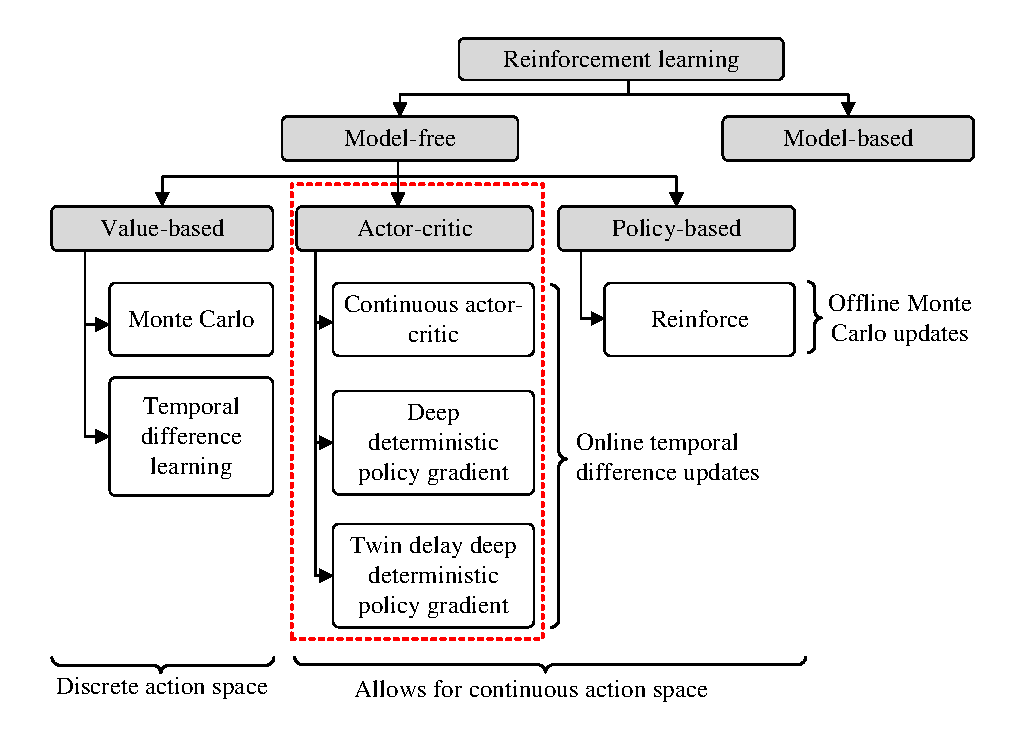
\includegraphics[width=\textwidth]{contents/chapt3/figs/reinforcement_learning_taxonomy.pdf}
\caption[A taxonomy of reinforcement learning algorithms]{A taxonomy of reinforcement learning algorithms. Beige blocks indicate general classes of methods, whereas blue indicates specific algorithms. The red dotted line encircles algorithms we applied and discuss in detail in this chapter.}
\label{fig:reinforcement_learning_taxonomy}
\end{figure}

\subsubsection{Value-based reinforcement learning}
\label{sec:value_based_rl}

Value-based reinforcement learning methods select actions by greedily maximising over an action-value function, 
\begin{equation}
    \pi(s) = \max_{a \in \mathcal{A}} q_\pi(s,a).
    \label{eq:greedy_policy}
\end{equation}
Since $q_\pi$ is an estimate of the return, this policy is expected to receive more reward than any other policy given the current action-values. The MDP is solved by iteratively improving the action-value estimate, then updating the policy based on the new value estimates until the condition for optimal action-value functions from Equation \ref{eq:q_*(s,a)} is met, at which point the greedy action selection in Equation \ref{eq:greedy_policy} is the optimal policy. The two step policy iteration process is described:

\begin{enumerate}
    \item The action-value function $q_\pi$ of the current policy $\pi$ is estimated by
    \begin{equation}
    \begin{split}
    Q_{\text{new}} & \leftarrow Q_{\text{old}} + \alpha \delta \\
    & \leftarrow \alpha [\text{target} - Q_{\text{old}}],
    \label{eq:Q_update}
    \end{split} 
    \end{equation}
    where $Q$ is an estimate of $q_\pi$ and $\delta$ is the update step. For now we assume the $Q$ is a lookup table, and handle the case where a neural network is used for function approximation in the next section.
    The action value-function must be predicted because the exact value of a policy is not initially known - the agent must first interact with the environment and sample rewards to get a good estimate of the return. 
    $Q$ is brought closer to $q_\pi$ by updating it towards the target, which is an updated estimate of the cumulative reward until the end of the episode. In Monte Carlo methods the target is $G_t$, sampled from Equation \ref{eq:q_pi(s,a)}:
    \begin{equation}
        Q(S_t, A_t) \leftarrow Q(S_t, A_t) + \alpha [\underbrace{G_t}_{\text{target}} - Q(S_{t}, A_{t})].
    \label{eq:monte_carlo_update}
    \end{equation}
    Using this target, the episode must be completed before $G_t$ is known, and thus the update is offline. Monte Carlo updates are slow and yield noisy target values. These issues are solved by temporal difference methods, who's targets are sampled from Equation \ref{eq:q_pi(s,a)_1}:
    \begin{equation}
        Q(S_t, A_t) \leftarrow Q(S_t, A_t) + \alpha [\underbrace{R_{t+1} + \gamma Q(S_{t+1}, A_{t+1})}_{\text{target}} - Q(S_{t}, A_{t})].
    \label{eq:td_update}
    \end{equation}
    The term $Q(S_{t+1}, A_{t+1})$ is referred to as a `bootstrapped estimate'. It provides an updated, readily available estimate of the return until the end of the episode, allowing for online implementation and updates at every time step. Furthermore, the variance of the target is reduced, and the algorithm learns better policies faster.
    The downside to using the bootstrapped estimate of the Q-value of the next state is that the target becomes biased. 
    \item After updating the action-value function, an improved policy based on $Q_{\text{new}}$ is generated by selecting the action with the maximum value with respect to the new action-values, 
    \begin{equation}
    \pi_{new}(s) = \max_{a \in \mathcal{A}} Q(s,a).
    \label{eq:new_greedy_policy}
    \end{equation}
\end{enumerate}
The process is iterative because the action-value function of the new policy generated in step two is unknown and needs to be estimated.
At each iteration,  $q_{\pi^{\text{new}}} \geq q_{\pi^{\text{old}}}$) until $q_\pi = q_*$, at which point $\pi = \pi_*$.

\subsubsection{Value-based reinforcement learning with neural network function approximiation}
\label{sec:value_rl_fnn}
We have assumed the value function to be a lookup table to simplify the discussion until now, and the theory must be adapted slightly for neural network value function approximation.
If the action-value function $Q$ is represented by an FNN parameterised by $\theta$, so that $Q(s, \theta) \approx Q(s)$, 
then there is a change to the action-value update rule in Equation \ref{eq:Q_update}. In the lookup table case, the update is to the entry in the table corresponding to state $S_t$. However, when an FNN is used, then the update is to the parameters of the FNN via a gradient descent step. As such, Equation \ref{eq:Q_update} is replaced by gradient descent Equation \ref{eq:gradient_descent}. The loss function to be minimised in the gradient descent step is then defined as the squared difference between the target and current learned action-values,
\begin{equation}
    \mathcal{L} = (\text{target} - Q(S_t, A_t,\theta_t))^2. 
\end{equation}
Even with the use of FNNs, the limitation on value-based methods is that the maximisation in step two requires that there be a finite number of actions available to the agent. We therefore turn our attention towards policy-based reinforcement learning in the next section.

\subsubsection{Policy-based reinforcement learning}
Policy-based methods are those that learn a parameterised policy, 
\begin{equation}
\pi(a|s,\theta) = \text{Pr}\{ A_t=a | S_t=s, \theta_t=\theta \}
\label{eq:policy_gradient_discrete_policy}
\end{equation}
for action selection. The policy is typically represented by an FNN with weight parameters $\theta$, which are learned by optimising a scalar performance measure $J(\theta)$ defined in terms of the state-value function $J(\theta) \doteq v_{\pi_\theta}(s_0)$. Therefore, gradient ascent in $J$ optimises performance and maximises the value function. The updates to the policy parameter are 
\begin{equation}
    \theta_{t+1} = \theta_t + \alpha  \nabla J(\theta_t).
    \label{eq:policy_update}
\end{equation}
This is similar to the gradient descent Equation \ref{eq:gradient_descent}, except $\nabla J(\theta)$ is added rather than subtracted.
Although the proof is not given here, the policy gradient theorem provides a useful expression for $\nabla J(\theta)$:
\begin{equation}
\begin{split}
    \nabla J(\theta) &\propto \sum_{s} \mu(s) \sum_{a} q_\pi(S_t, a) \nabla \pi (a | s, \theta) \\
    &= \mathbb{E}_\pi \left[ G_t   \nabla \ln \pi (A_t | S_t, \theta) \right]
    \label{eq:policy_gradient}
\end{split}
\end{equation}
where $\mu$ is the on-policy state distribution under policy $\pi$. By sampling the expectation from Equation \ref{eq:policy_gradient} and adjusting for a baseline chosen as the estimated state-value function $V(S_t)$ the update to the policy is 
\begin{equation}
\begin{split}
    \theta_{t+1} &= \theta_{t} + \alpha \delta \nabla \ln \pi(A_t | S_t, \theta_t) \\
    &= \theta_{t} + \alpha ( \text{target} - V(S_t) ) \nabla \ln \pi(A_t | S_t, \theta_t) \\
    &= \theta_{t} + \alpha ( G_t - V(S_t) ) \nabla \ln \pi(A_t | S_t, \theta_t).
    \label{eq:reinforce_update}
\end{split}
\end{equation}
The value function in any policy-based method is estimated using a value-based update step from Section \ref{sec:value_based_rl}. In this case, a state-value function $V$ is utilised, and the target $G_t$ is selected to reflect the policy update. This is equivalent to sampling from Equation \ref{eq:v_pi(s)},
\begin{equation}
    V(S_t) \leftarrow V(S_t) + \alpha [G_t - V(S_{t})].
    \label{eq:monte_carlo_v_update}
\end{equation}
This is the update for the classic REINFORCE algorithm. The algorithm is analogous to the value-based Monte Carlo methods in that it bases the policy update on the entire episode's return $G_t$, requiring that the updates only occur after an episode completes. 
We find that REINFORCE has similar pitfalls as the value-based Monte Carlo methods.
However, methods that use the estimated value of the next state rather than the full return, such as temporal difference learning from the value-based methods are often superior to those that use the full episode return in the update step. 
Methods that use such an update step whilst maintaining a parameterised policy are \emph{actor-critics}.

\subsubsection{Actor-critic reinforcement learning}
Actor-critics, so called because they maintain both a parameterised policy (actor) and value-function (critic) are policy-gradient methods that utilise a temporal difference update step.
The updates to the policy is analogous to Equation \ref{eq:reinforce_update}, except that the $G_t$ term in the target is replaced by a sample from Equation \ref{eq:v_pi(s)_1}. That is, the current reward summed with a bootstrapped estimate of the value of the next state:
\begin{equation}
    \theta_{t+1} = \theta_{t} + \alpha ( \underbrace{R_{t+1} + V(S_{t+1})}_{\text{target}} - V(S_t) ) \nabla \ln \pi(A_t | S_t, \theta_t),
    \label{eq:actor_critic_update}
\end{equation}
The target to the update in the state-value function from Equation \ref{eq:monte_carlo_v_update} is also modified in the same way,
\begin{equation}
    V(S_t) \leftarrow V(S_t) + \alpha [\underbrace{R_{t+1} + V(S_{t+1})}_{\text{target}} - V(S_{t})].
    \label{eq:actor_critic_v_update}
\end{equation}
This modification to the target allows for online implementation,
resulting in the similar benefits as in the value-based reinforcement learning case, 
namely reduced variance on the target and higher efficiency.
We now introduce an algorithm that makes a modification to the standard actor-critic method that allows for continuous action spaces.

\subsubsection{Continuous actor-critic}
\label{sec:cont_act_crit}

We present an implementation of the continuous actor-critic algorithm with an FNN state-value function approximator parameterised by $\theta$, $V_{\theta} \cong V$.
The policy $\pi_\phi$, chosen to be a FNN with parameters $\phi$, outputs the statistics of a gaussian distribution rather than the probabilities of selection each action. The action is selected by sampling from this distribution,
\begin{equation}
    a \sim \pi_{\phi}(a|s) = \mathcal{N}(\mu(s,\phi), \sigma(s,\phi)).
\label{eq:act_crit_act}
\end{equation}
The pseudocode for continuous actor-critic is shown in Algorithm \ref{alg:cont_act_crit}. Notice that the agent-environment interaction described by the inner for-loop matches the structure of the MDP given in Section \ref{sec:agent_environment_interface}. 
Once the actor, critic and environment are initialised, $M$ episodes are run.
The agent and environment interact at every time step in an episode: the agent samples a state, selects an action to be executed, then observes the reward and next state. This is followed by an update to the actor and critic. 
Since neural network function approximation is used, the modifications in Section \ref{sec:value_rl_fnn} are applied to the state-value update Equation \ref{eq:actor_critic_v_update} to achieve a gradient descent update step. The loss for the gradient descent step at time step $t$ is given by
\begin{equation}
    \delta_t = (r_t + \gamma V_\theta(S_{t+1}) - V_\theta(S_t))^2.
\end{equation}
Furthermore, the actor policy is updated using the gradient ascent step from Equation \ref{eq:actor_critic_update}, the loss for which is
\begin{equation}
    L_\phi = - \delta_t \ln(\pi_\phi(S_t)).
\end{equation}
Notice that the loss is taken as the negative of the update step; this is because in practice gradient ascent is achieved by calling a gradient descent function with a negative loss argument.

\begin{algorithm}[hbt!]
\caption{Continuous actor-critic}\label{alg:cont_act_crit}
Initialise critic $V_{\theta}(s)$ and actor network $\pi_{\phi}(s)$ with weights $\theta$ and $\phi$ respectively\\
Initialise the environment\\
\For{episode = 1, M}
{
    Receive initial observation state $s_0$\\
    \For{t=0, T}
    {
        $\text{Sample action } a_t = \pi_{\phi}(S_t)$ \\
        Execute $a_t$, observe next state $S_{t+1}$ and reward $r$    \\
        Set TD target: $y_t = r + \gamma \cdot V_{\theta}(S_{t+1})$ \\
        Update critic (state-value function) by minimizing loss: $\delta_t = (y_t - V_{\theta}(S_t))^2$ \\
        Update actor policy by minimising loss: \hspace{5cm}
        $L_\phi = -\delta_t \ln(\pi_{\phi}(S_t))$ \\
        Update $S_t \leftarrow S_{t+1}$\\
    }
}
\end{algorithm}

A disadvantage to this algorithm is that it discards state transitions after learning from them only once.
However, training can be made more efficient and stable by basing the training update on multiple sampled experiences using an experience replay buffer.
Furthermore, Silver et al. \cite{silver2014} show that the stochastic policy in Equation \ref{eq:act_crit_act} is less sample efficient than a deterministic policy. We thus move on to deterministic policy gradient algorithms in the next section. 

\subsubsection{Deep deterministic policy gradient}

The deterministic policy gradient (DPG) proposed by Silver et al. \cite{silver2014} is an off-policy actor-critic method for continuous action spaces. 
Off-policy refers to algorithms that learn a target policy from an exploratory behaviour policy. 
Thus the target policy is a function that deterministically maps states to actions, $a_t = \pi(s_t)$.
The behaviour policy that the agent follows while interacting with the environment is then the target policy with noise, 
\begin{equation}
    a_t = \pi_{\phi}(s_t) + \mathcal{N}_t,
\end{equation}
where $\mathcal{N_t}$ is the noise process.
Since DDPG is an actor-critic method, the policy is updated according to a gradient ascent step. 
As such, Silver et al. \cite{silver2014} present the deterministic policy gradient, analogous to the policy gradient for stochastic policies presented in Equation \ref{eq:policy_gradient}:
\begin{equation}
\begin{split}
    \nabla_{\phi} J(\phi) &\approx \mathbb{E}[ \nabla_{\phi} Q_{\theta}(s,a) |_{s=s_t, a=\pi_{\phi}(s_t)}]\\
    &= \mathbb{E} [ \nabla_{a} Q_{\theta}(s,a)|_{s=s_t, a=\pi_{\phi}(s_t)} \nabla_{\phi} \pi_{\phi}(s)|_{s=s_t}],
    \label{eq:deterministic_policy_gradient}
    \end{split}
\end{equation}
where the actor policy $\pi_{\phi}$ and action-value function $Q_{\theta}$ are parameterised by $\phi$ and $\theta$ respectively. Equation \ref{eq:deterministic_policy_gradient} states that the gradient of the cost function $\phi$ is the gradient of the action-value function with respect to the policy parameters. Practically this is achieved by setting the loss of the cost function $J(\phi)$ equal to the action-value of a state and and action determined by the target policy.
While Silver et al. \cite{silver2014} apply this update rule to a linear function approximator case, Lillicrap et al. \cite{Lillicrap2016} make the necessary modifications for neural network function approximation in their algorithm named deep deterministic policy gradient (DDPG). 
The pseudo code for DDPG is shown in Algorithm \ref{alg:ddpg}. 
Its structure is similar to the continuous actor-critic Algorithm \ref{alg:cont_act_crit}, but with modifications that improve performance over standard actor-critic and account for deterministic action selection.

The DDPG algorithm makes use of an idea introduced by Lin \cite{lin1993}, the experience replay buffer. At each time step $t$, the agent's experience $e_t = (s_t,a_t,r_t,s_{t+1})$ is stored in a data set $\mathcal{B} = e_1, e_2, ... , e_N$. 
The learning step is then applied to random samples of the replay buffer, $e \sim \mathcal{D}$. 
Maintaining a history of experiences allows each experience to potentially be used for several weight updates.
This results in greater data efficiency, reduces the variance of the updates by breaking correlations between samples, and prevents the neural network parameters from getting stuck in local minima \cite{mnih2013}.

Another issue that DDPG addresses is that of training stability: in continuous actor-critic, the current value estimate is updated towards a target which changes at every time step, potentially causing it to become unstable. This issue is addressed by maintaining two actor-critic pairs. The first pair is updated continually, while the second pair, referred to as the target actor and critic because they are used to calculate the target to the critic update, are changed at a much slower rate using a soft update rule.
The target for the update to the critic is then calculated using sampled state transitions from the replay buffer:
\begin{equation}
    y_i = r_i + \gamma Q_{\theta'}(s_{i+1}, \pi_{\theta'}(s_{i+1})),
\end{equation}
where $s_{i+1}$ are sampled states, and $Q_{\theta'}$ and $\pi_{\theta'}$ are the target actor and critic respectively. Since a neural network is used, the critic update step is a gradient descent step with the cost function set equal to the mean squared error between the target values for the sampled transitions and their action-values evaluated by the current network,
\begin{equation}
    L_{\theta}=\frac{1}{N} \sum_i (y_i - Q_{\theta}(s_i,a_i))^2.
\end{equation}
The soft update to the target action-value and policy parameters $\theta'$ and $\phi'$ are given by
\begin{equation}
\begin{split}
    \theta' &\leftarrow \tau \theta' + (1 - \tau) \theta, \\
    \phi' &\leftarrow \tau \phi + (1 - \tau) \phi'.
\end{split}
\end{equation}
where $\tau \ll 1$. This prevents the target from changing too quickly, stabilising the learning step. 
At the time of its release, DDPG was a state of the art model-free technique for continuous action spaces, 
even being competitive with algorithms which have full access to the dynamics model.
However, there are improvements to be made: Overestimation bias, whereby a state with a low actual value is approximated as having a high action-value is an issue identified by Fujimoto et al. \cite{Fujimoto2018}.
The next section introduces an algorithm that makes improvements over DDPG by addressing value overestimation.

\begin{algorithm}[htb!]
\caption{Deep deterministic policy gradient}\label{alg:ddpg}
Initialise critic network $Q_{\theta}(s,a)$ and actor $\pi_{\phi}(s)$ with weights $\theta$ and $\phi$ \\
Initialise target network $Q_{\theta'}$ and $\pi_{\phi'}$ with weights $\theta' \leftarrow \theta$, $\phi' \leftarrow \phi$ \\
Initialise replay buffer $\mathcal{B}$ \\
\For{episode = 1, M}
{
    Initialise a random noise process $\mathcal{N}$ for action exploration \\
    Receive initial observation state $s_0$\\
    \For{t=0, T}
    {
        $\text{Select action } a_t = \pi_{\phi}(s_t) + \mathcal{N}_t$\\
        Execute action $a_t$, observe reward $r_t$, observe new state $s_{t+1}$ \\
        Store transition $(s_t, a_t, r_t, s_{t+1})$ in $\mathcal{B}$ \\
        Sample a random minibatch of $N$ transitions $(s_i, a_i, r_i, s_{i+1})$ from $\mathcal{B}$ \\
        Set TD target: $y_i = r_i + \gamma Q_{\theta'}(s_{i+1}, \pi_{\phi'}(s_{i+1}))$ \\
        Update critic by minimising the loss: $L_{\theta}=\frac{1}{N} \sum_i (y_i - Q_{\theta}(s_i,a_i))^2 $ \\
        Update the actor policy using the sampled policy gradient:
        $\nabla_{\phi} J \approx \frac{1}{N} \sum_i \nabla_{a} Q_{\theta}(s,a)|_{s=s_t, a=\pi{\phi}(s_t)} \nabla_{\phi} \pi_{\phi}(s)|_{s=s_t} $\\
        Update the target networks:\\
        $\theta' \leftarrow \tau \theta' + (1 - \tau) \theta$\\
        $\phi' \leftarrow \tau \phi + (1 - \tau) \phi'$\\
    }
}
\end{algorithm}


\subsection{Twin delay deep deterministic policy gradient}

The twin delay deep deterministic policy gradient (TD3) presented by Fujimoto et al. \cite{Fujimoto2018} is a modification to DDPG that addresses overestimation of action-values as a result of using function approximators as well as high variance in the critic update.
Action-value overestimation is an issue since it may develop into a significant bias over many update steps, and may lead to poor quality policies \cite{hasselt2015}.
Likewise, variance in the critic update produces poor quality policies and slows learning.
TD3 maintains the target networks, experience replay buffer, action selection mechanism and actor update from DDPG, with a few key differences shown in Algorithm \ref{alg:td3}.

\begin{algorithm}[hbt!]
\caption{Twin delay deep deterministic policy gradient}\label{alg:td3}
Initialise critic networks $Q_{\theta_1}, Q_{\theta_2}$ and actor network $\pi_\phi$ 
with parameters $\theta_1, \theta_2$ and $\pi_\phi$ \\
Initialise target networks $Q_{\theta_1'}$, $Q_{\theta_2'}$ and $\pi_{\phi'}$ with weights 
$\theta_1' \leftarrow \theta_1$, $\theta_2' \leftarrow \theta_2$, and $\phi' \leftarrow \phi$ \\
Initialise experience replay buffer $\mathcal{B}$ \\
\For{episode = 1, M}
{

    \For{t=0, T}
    {
        Select an action with random exploration noise $a \sim \pi_{\phi}(s) + \epsilon$, $\epsilon \sim \mathcal{N}(0, \sigma)$ \\
        Observe reward $r$ and new state $s_{t+1}$ \\
        Store transition tuple $(s_t,a_t,r_t,s_{t+1})$ in $\mathcal{B}$ \\
        
        Sample mini-batch of $N$ transitions $(s_i,a_i,r_i,s_{i+1})$ from $\mathcal{B}$ \\
        Select target actions: \hspace{5cm}
        $\tilde{a} \leftarrow \pi_{\phi'}(s_{t+1}) + \epsilon$, $\epsilon \sim \text{clip}(\mathcal{N}(0,\tilde{\sigma}), -c,c)$ \\
        Set TD target: \hspace{5cm}
        $y \leftarrow r + \gamma \min_{i=1,2} Q_{\theta_i'}(s_{t+1}, \tilde{a})$ \\
        Update critics by minimising the loss: \hspace{5cm}
        $L_{\theta_i} \leftarrow  \frac{1}{N} \sum (y - Q_{\theta_i}(s,a))^{2} $ \\
        \If{$t \text{ mod } d$}
        {
            Update $\phi$ by the deterministic policy gradient:
            $\nabla_\phi J(\phi) = \frac{1}{N} \sum \nabla_a Q_{\theta_1} (s,a) | _{a=\theta_\phi(s)} \nabla_\phi \pi_\phi(s)$ \\
            Update target networks: \\
            $\theta_{i}' \leftarrow \tau \theta_i + (1 - \tau) \theta_{i}'$ \\
            $\phi' \leftarrow \tau \phi + (1 - \tau) \theta'$ \\
        }
    }
}
\end{algorithm}

Fujimoto et al. \cite{Fujimoto2018} address the issue of variance in the target of the critic update by introducing a regularisation strategy, to add small amount of noise $\mathcal{N}$ to the target action $\tilde{a}$, which smooths the value estimate.
Thus, action which is evaluated for the critic update is
\begin{equation}
    \tilde{a} \leftarrow \pi_{\phi'}(s_{t+1}) + \epsilon, \epsilon \sim \text{clip}(\mathcal{N}(0,\tilde{\sigma}), -c,c).
\end{equation}
Furthermore, to combat value overestimation, Fujimoto et al. \cite{Fujimoto2018} adapt double Q-learning from Hasselt et al. \cite{hasselt2015} for deterministic policy gradients. 
In double Q-learning, two action-value functions $Q_{\theta_1}$ and $Q_{\theta_2}$ are maintained
, allowing two independent targets to be calculated using both action-value functions at every time step.
Both critics are then updated towards the target containing the minimum of their two estimated action values:
\begin{equation}
    y \leftarrow r + \gamma \min_{i=1,2} Q_{\theta_i'}(s_{t+1}, \hat{a}).
\end{equation}
Although this may result in action-value underestimation, this is considered less severe than overestimation.
Overall, the addition of double Q-learning stabilises and results in more reliable learning.
The final modification that TD3 makes to DDPG is to update the policy and target networks only every $d$ time steps to minimise the likelihood of repeating policy  updates with respect to an unchanged critic.
To the best of our knowledge, TD3 is the state of the art in continuous action space reinforcement learning, outperforming DDPG and continuous actor-critic in a variety of benchmarks.

\subsection{Summary}
In this chapter, we have summarised the core concepts for implementing reinforcement learning techniques, namely Markov decision processes, function approximators, and the reinforcement learning techniques themselves.
The Markov decision process was introduce first as the precise mathematical problem that reinforcement learning tries to solve in a computationally tractable manner.
Function approximation was then introduced to handle cases where the state space is too large for each state to be represented independently of each other, a necessary requirement to make Markov decision processes and reinforcement learning realisable.
The focus was on deep neural networks due to their ability to approximate highly non-linear functions. In fact, very few learning approaches for autonomous racing use function approximators other than neural networks.
We then presented an overview of the field of reinforcement learning, highlighting the differences between value-based techniques, policy-based techniques and actor-critic. 
We summarise three actor-critic algorithms, which is our method of choice for this project: continuous actor-critic, deep deterministic policy gradient, and twin delay deep deterministic policy gradient.
Table \ref{table:rl_summary} shows a short summary of the discussion and decision criteria for method selection. 
In the next chapter, we will see how the theory presented here is used to create a simulation that can train an agent to successfully race around a track.

\newcolumntype{L}{>{\raggedleft\arraybackslash}p{6cm}}
\newcolumntype{M}{>{\centering\arraybackslash}p{2.8cm}}
\newcolumntype{R}{>{\centering\arraybackslash}p{1.8cm}}

\begin{table}[h]
\centering
\renewcommand{\arraystretch}{1.1}
\begin{tabularx}{0.85\textwidth} {LMR}
    \hline
    \textbf{Method} & \textbf{continuous action space} & \textbf{online} \\
    \hline
    Value-based, Monte Carlo  &  &   \\
    Value-based, temporal difference  &  & \checkmark  \\
    Policy-based & \checkmark &  \\
    Actor-critic & \checkmark & \checkmark \\
    \hline
\end{tabularx}
\caption[Criteria for reinforcement learning method selection]{A condensed decision criteria for reinforcement learning method selection.}
\label{table:rl_summary}
\end{table}
